\documentclass[12pt]{article}

\usepackage{fullpage}
\usepackage{multicol,multirow}
\usepackage{tabularx}
\usepackage{ulem}
\usepackage[utf8]{inputenc}
\usepackage[russian]{babel}
\usepackage{graphicx}
\usepackage{indentfirst}


\begin{document}

\section*{Лабораторная работа №\,3 по курсу дискрeтного анализа: исследование качества программы}

Выполнил студент группы М08-207Б МАИ \textit{Цапков Александр}.

\subsection*{Условие}

\begin{enumerate}
\item Для реализации словаря из предыдущей лабораторной работы необходимо провести исследование скорости выполнения и потребления оперативной памяти. В случае выявления ошибок или явных недочётов, требуется их исправить.
Результатом лабораторной работы является отчёт, состоящий из:
Дневника выполнения работы, в котором отражено что и когда делалось, какие сред- ства использовались и какие результаты были достигнуты на каждом шаге выпол- нения лабораторной работы.
Выводов о найденных недочётов.
Сравнение работы исправленной программы с предыдущей версии. Общих выводов о выполнении лабораторной работы, полученном опыте.
Минимальный набор используемых средст должен содержать утилиту gprof и биб- лиотеку dmalloc, однако их можно заменять на любые другие аналогичные или более известные утилиты (например, Valgrind или Shark) или добавлять к ним новые (на- пример, gcov).
\end{enumerate}

\subsection*{Общий подход}

При выполнении своей лабараторной работы я использовал следующие утилиты: Valgrind-- для выявления ошибок работы с памятью, Valgrind c callgrind как профилирофщик, kcachegrind-- для визуализации данных полученных с помощью callgrind, LLDB-- как отладчик обычных ошибок и DrMemory для выявления работы с памятью в macOS (так как там не работает valgrind).

\subsection*{Разбор используемых утилит}

LLDB-- "высокопроизводительный отладчик. Он сделан как множество повторно используемых компонентов широко использующих существующие библиотеки проекта LLVM, к примеру, парсер выражений Clang или дизассемблер LLVM."

Его синтаксис очень похож на синтаксис всем известного GDB. Мой выбор пал именно на LLDB из-за его совместимости с macOS, тогда как GDB у меня запустить не получилось.


Valgrind — "инструментальное программное обеспечение, предназначенное для отладки использования памяти, обнаружения утечек памяти, а также профилирования. Название valgrind взято из германо-скандинавской мифологии, где является названием главного входа в Вальгаллу."


Валгринд способен не только утечки памяти, но и ошибки работы с нею, такие как запись и чтение неинициализированные переменных, уже освобожденной памяти и т.п. Его интерфейс показывает трэйсбэк вызова где произошла ошибка, однако в macOS я пользовался утилитой DrMrmory, которая находится в альфа версии на macOS и работает очень медленно, однако вывод у нее гозаздо более понятный и при компиляции с флагом -g показывает строки которые вызвали эту ошибку.

Вот листинг теста на утечки о ошибки памяти уже готовой программы.

\begin{lstlisting}
root@Kali:~/Documents/Study/Labs/DA/sem3da/2lr(4)/solution# ls
BTree.hpp  List.hpp  main.cpp  Makefile  Vector.hpp
root@Kali:~/Documents/Study/Labs/DA/sem3da/2lr(4)/solution# make
g++ -Wall -pedantic -std=c++11 main.cpp -o solution
root@Kali:~/Documents/Study/Labs/DA/sem3da/2lr(4)/solution# cat ../generated.tst | valgrind ./solution > /dev/null
==4337== Memcheck, a memory error detector
==4337== Copyright (C) 2002-2017, and GNU GPL'd, by Julian Seward et al.
==4337== Using Valgrind-3.15.0 and LibVEX; rerun with -h for copyright info
==4337== Command: ./solution
==4337== 
==4337== 
==4337== HEAP SUMMARY:
==4337==     in use at exit: 122,880 bytes in 6 blocks
==4337==   total heap usage: 1,407,226 allocs, 1,407,220 frees, 203,038,216 bytes allocated
==4337== 
==4337== LEAK SUMMARY:
==4337==    definitely lost: 0 bytes in 0 blocks
==4337==    indirectly lost: 0 bytes in 0 blocks
==4337==      possibly lost: 0 bytes in 0 blocks
==4337==    still reachable: 122,880 bytes in 6 blocks
==4337==         suppressed: 0 bytes in 0 blocks
==4337== Rerun with --leak-check=full to see details of leaked memory
==4337== 
==4337== For lists of detected and suppressed errors, rerun with: -s
==4337== ERROR SUMMARY: 0 errors from 0 contexts (suppressed: 0 from 0)
\end{lstlisting}

Callgrind является частью Valgrind'а. Valgrind запускает программу «в песочнице», фактически используя виртуализации. Callgrind производит профилирование основываясь на брейкпоинтах на инструкциях типа call и ret. Он значительно замедляет анализируемый код, как правило, от 5 до 20 раз. Таким образом, для анализа на больших данных в runtime он, как правило, не годен.
Однако инструмент очень популярен, и простой формат графа вызовов поддерживается отличными средствами визуализации, например, kcachegrind, которым я и воспользовался. Приемущество для меня в хорошо предствавленных данных, с помощью которого можно легко найти проблемы. И не просто легко но и мощьно, callgrind предостовляет множество полезных данных, а kcachegrind позволяет ими легко прерировать.

Вот пример сбора данных с callgrind. 

\begin{lstlisting}
root@Kali:~/Documents/Study/Labs/DA/sem3da/2lr(4)/solution# valgrind --tool=callgrind ./solution < ../generated.tst > /dev/null
==4395== Callgrind, a call-graph generating cache profiler
==4395== Copyright (C) 2002-2017, and GNU GPL'd, by Josef Weidendorfer et al.
==4395== Using Valgrind-3.15.0 and LibVEX; rerun with -h for copyright info
==4395== Command: ./solution
==4395== 
==4395== For interactive control, run 'callgrind_control -h'.
==4395== brk segment overflow in thread #1: can't grow to 0x482e000
==4395== (see section Limitations in user manual)
==4395== NOTE: further instances of this message will not be shown
==4395== 
==4395== Events    : Ir
==4395== Collected : 6883812082
==4395== 
==4395== I   refs:      6,883,812,082
\end{lstlisting}

Kcachegrind-- Используется для визуализации вывода callgrind и других профилировщиков с таким же форматом вывода. 
Очень наглядно и интерактивно показывает нам данные. В своей ЛР я пользовался именнно связкой calgrind--kcachegrind.

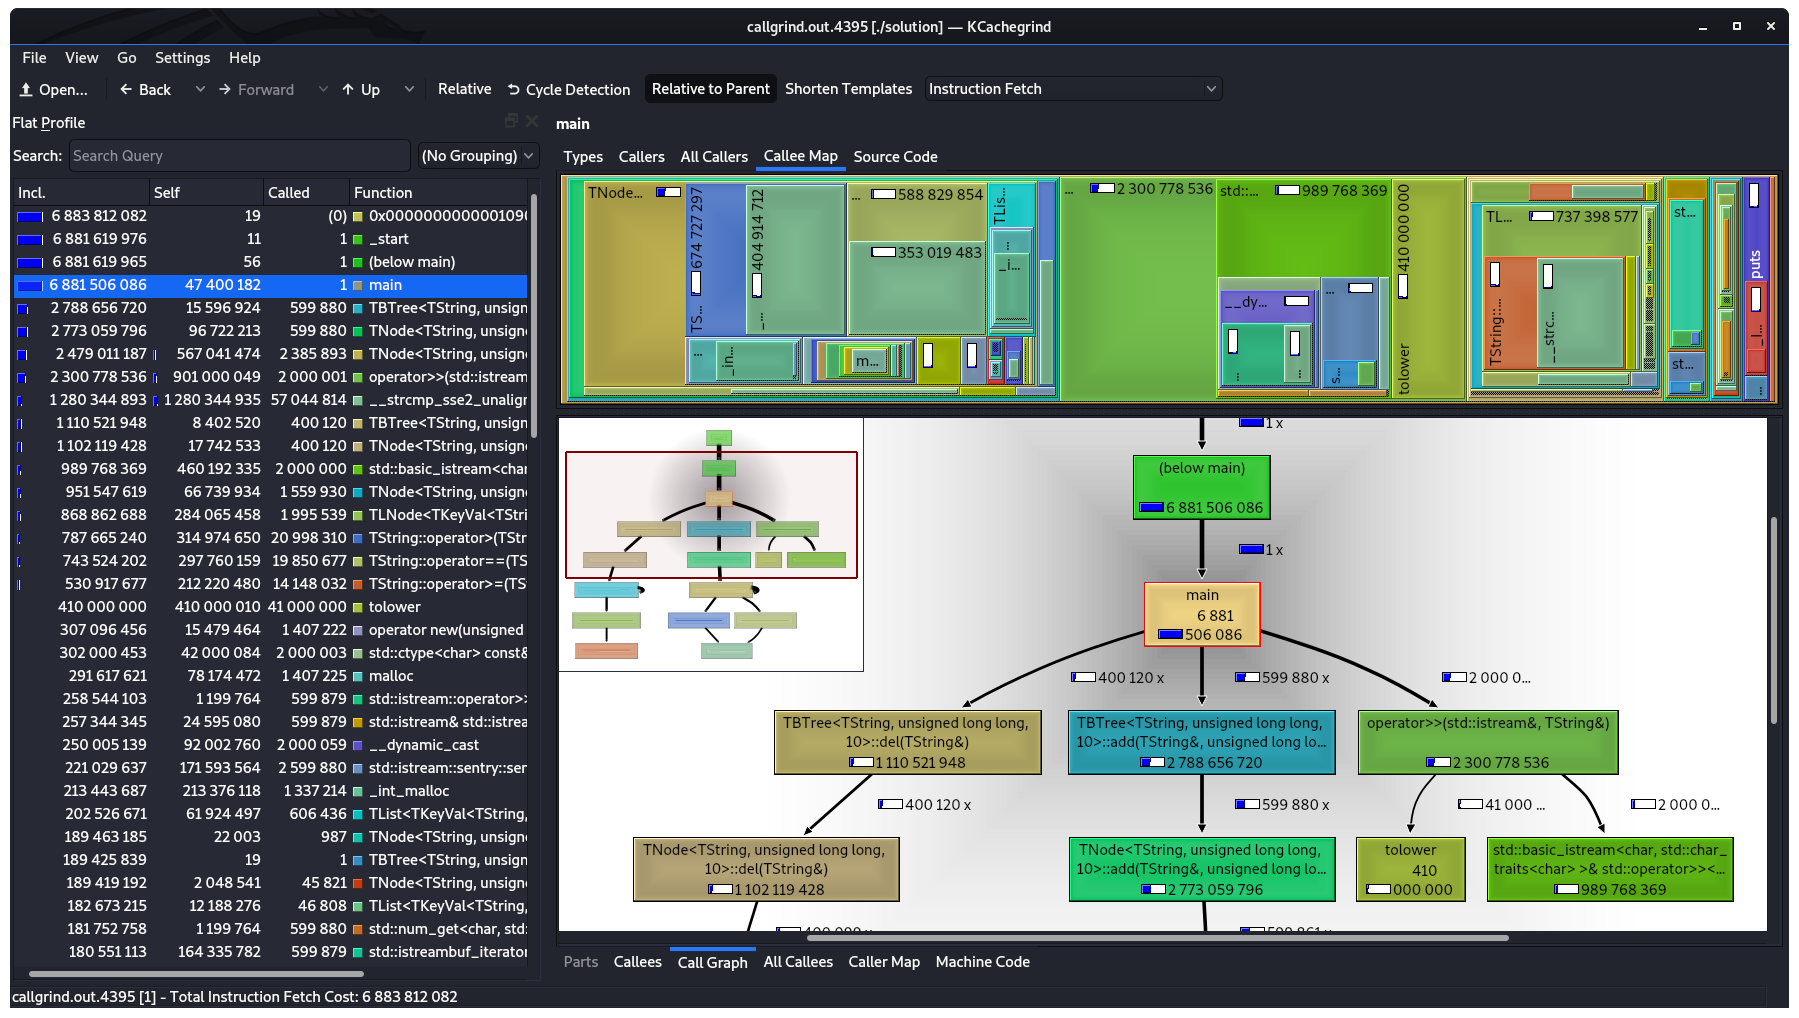
\includegraphics[width=\linewidth]{callgrind}

Также "каноном" профилировщиков считается perv и fprof, но я нахожу callgrind более удобным для личного пользования. perv, также как callgrind работает в 2 этапа: c,jh byajhvfwbb b tt dsdjl (record и report).

\subsection*{Дневник этапов написания программы}

1.Написал основную структуру дерева и лист. Проверял вручную правильность работы листа.

2.Написал вставку в дерево вообще нигде не используя delete. Впервые воспользовался отладчиком lldb.

3.После вставки решил заняться удалением. Прежде чем писать удаление написал ко всему диструкторы и проверил в 
первый раз и отладил все с помощью valgrinda.

4.Реализовал удаление, исправил ошибки с очищением памяти, написал свою менюшку и стринг для того чтобы проверить на чекере. Ошибка выполнения.

5.С помощью lldb и много часов выяснил проблему. Удаление и вставка завершены.

6.Написал сохранение и загрузку дерева. Проверил valgrind'ом и исправил неинициализированные переменные.

7.Все было готово но тайм лимит на 13 тесте. После нескольких дней поисков решения воспользовался профилировщиком 
callgrind и сразу нашел и исправил свой недачет. Программа ускорила свою работу в 3 раза.


\subsection*{Выводы}

Без этой лабараторной работы я бы, скорее всего, до сих пор бы не сделал 2-ю. Я не знал что такое профилировщики и когда узнал (это было как раз во время тайм лимита), проверил свою программу и мгновенно нашел ошибку. Кроме того для выполнения таких, достаточно больших лабараторных и каких-либо проектов в будующем практически необходимо пользоваться всем что может облегчить жизнь программисту. К примеру я раньше использовал отладочные принты для поиска ошибок, но для 2-й лр я специально потратил час на изучение основ LLDB, что в разы упростило всю мою работу.

\end{document}

